% Options for packages loaded elsewhere
\PassOptionsToPackage{unicode}{hyperref}
\PassOptionsToPackage{hyphens}{url}
%
\documentclass[
]{article}
\title{Final Reflection}
\author{Anna Repesh}
\date{12/2/2021}

\usepackage{amsmath,amssymb}
\usepackage{lmodern}
\usepackage{iftex}
\ifPDFTeX
  \usepackage[T1]{fontenc}
  \usepackage[utf8]{inputenc}
  \usepackage{textcomp} % provide euro and other symbols
\else % if luatex or xetex
  \usepackage{unicode-math}
  \defaultfontfeatures{Scale=MatchLowercase}
  \defaultfontfeatures[\rmfamily]{Ligatures=TeX,Scale=1}
\fi
% Use upquote if available, for straight quotes in verbatim environments
\IfFileExists{upquote.sty}{\usepackage{upquote}}{}
\IfFileExists{microtype.sty}{% use microtype if available
  \usepackage[]{microtype}
  \UseMicrotypeSet[protrusion]{basicmath} % disable protrusion for tt fonts
}{}
\makeatletter
\@ifundefined{KOMAClassName}{% if non-KOMA class
  \IfFileExists{parskip.sty}{%
    \usepackage{parskip}
  }{% else
    \setlength{\parindent}{0pt}
    \setlength{\parskip}{6pt plus 2pt minus 1pt}}
}{% if KOMA class
  \KOMAoptions{parskip=half}}
\makeatother
\usepackage{xcolor}
\IfFileExists{xurl.sty}{\usepackage{xurl}}{} % add URL line breaks if available
\IfFileExists{bookmark.sty}{\usepackage{bookmark}}{\usepackage{hyperref}}
\hypersetup{
  pdftitle={Final Reflection},
  pdfauthor={Anna Repesh},
  hidelinks,
  pdfcreator={LaTeX via pandoc}}
\urlstyle{same} % disable monospaced font for URLs
\usepackage[margin=1in]{geometry}
\usepackage{color}
\usepackage{fancyvrb}
\newcommand{\VerbBar}{|}
\newcommand{\VERB}{\Verb[commandchars=\\\{\}]}
\DefineVerbatimEnvironment{Highlighting}{Verbatim}{commandchars=\\\{\}}
% Add ',fontsize=\small' for more characters per line
\usepackage{framed}
\definecolor{shadecolor}{RGB}{248,248,248}
\newenvironment{Shaded}{\begin{snugshade}}{\end{snugshade}}
\newcommand{\AlertTok}[1]{\textcolor[rgb]{0.94,0.16,0.16}{#1}}
\newcommand{\AnnotationTok}[1]{\textcolor[rgb]{0.56,0.35,0.01}{\textbf{\textit{#1}}}}
\newcommand{\AttributeTok}[1]{\textcolor[rgb]{0.77,0.63,0.00}{#1}}
\newcommand{\BaseNTok}[1]{\textcolor[rgb]{0.00,0.00,0.81}{#1}}
\newcommand{\BuiltInTok}[1]{#1}
\newcommand{\CharTok}[1]{\textcolor[rgb]{0.31,0.60,0.02}{#1}}
\newcommand{\CommentTok}[1]{\textcolor[rgb]{0.56,0.35,0.01}{\textit{#1}}}
\newcommand{\CommentVarTok}[1]{\textcolor[rgb]{0.56,0.35,0.01}{\textbf{\textit{#1}}}}
\newcommand{\ConstantTok}[1]{\textcolor[rgb]{0.00,0.00,0.00}{#1}}
\newcommand{\ControlFlowTok}[1]{\textcolor[rgb]{0.13,0.29,0.53}{\textbf{#1}}}
\newcommand{\DataTypeTok}[1]{\textcolor[rgb]{0.13,0.29,0.53}{#1}}
\newcommand{\DecValTok}[1]{\textcolor[rgb]{0.00,0.00,0.81}{#1}}
\newcommand{\DocumentationTok}[1]{\textcolor[rgb]{0.56,0.35,0.01}{\textbf{\textit{#1}}}}
\newcommand{\ErrorTok}[1]{\textcolor[rgb]{0.64,0.00,0.00}{\textbf{#1}}}
\newcommand{\ExtensionTok}[1]{#1}
\newcommand{\FloatTok}[1]{\textcolor[rgb]{0.00,0.00,0.81}{#1}}
\newcommand{\FunctionTok}[1]{\textcolor[rgb]{0.00,0.00,0.00}{#1}}
\newcommand{\ImportTok}[1]{#1}
\newcommand{\InformationTok}[1]{\textcolor[rgb]{0.56,0.35,0.01}{\textbf{\textit{#1}}}}
\newcommand{\KeywordTok}[1]{\textcolor[rgb]{0.13,0.29,0.53}{\textbf{#1}}}
\newcommand{\NormalTok}[1]{#1}
\newcommand{\OperatorTok}[1]{\textcolor[rgb]{0.81,0.36,0.00}{\textbf{#1}}}
\newcommand{\OtherTok}[1]{\textcolor[rgb]{0.56,0.35,0.01}{#1}}
\newcommand{\PreprocessorTok}[1]{\textcolor[rgb]{0.56,0.35,0.01}{\textit{#1}}}
\newcommand{\RegionMarkerTok}[1]{#1}
\newcommand{\SpecialCharTok}[1]{\textcolor[rgb]{0.00,0.00,0.00}{#1}}
\newcommand{\SpecialStringTok}[1]{\textcolor[rgb]{0.31,0.60,0.02}{#1}}
\newcommand{\StringTok}[1]{\textcolor[rgb]{0.31,0.60,0.02}{#1}}
\newcommand{\VariableTok}[1]{\textcolor[rgb]{0.00,0.00,0.00}{#1}}
\newcommand{\VerbatimStringTok}[1]{\textcolor[rgb]{0.31,0.60,0.02}{#1}}
\newcommand{\WarningTok}[1]{\textcolor[rgb]{0.56,0.35,0.01}{\textbf{\textit{#1}}}}
\usepackage{graphicx}
\makeatletter
\def\maxwidth{\ifdim\Gin@nat@width>\linewidth\linewidth\else\Gin@nat@width\fi}
\def\maxheight{\ifdim\Gin@nat@height>\textheight\textheight\else\Gin@nat@height\fi}
\makeatother
% Scale images if necessary, so that they will not overflow the page
% margins by default, and it is still possible to overwrite the defaults
% using explicit options in \includegraphics[width, height, ...]{}
\setkeys{Gin}{width=\maxwidth,height=\maxheight,keepaspectratio}
% Set default figure placement to htbp
\makeatletter
\def\fps@figure{htbp}
\makeatother
\setlength{\emergencystretch}{3em} % prevent overfull lines
\providecommand{\tightlist}{%
  \setlength{\itemsep}{0pt}\setlength{\parskip}{0pt}}
\setcounter{secnumdepth}{-\maxdimen} % remove section numbering
\ifLuaTeX
  \usepackage{selnolig}  % disable illegal ligatures
\fi

\begin{document}
\maketitle

\hypertarget{final-project-update}{%
\subsection{Final Project update}\label{final-project-update}}

\url{https://github.com/arepesh/Final-Project}

Bella and I have been working on this project together. This link goes
to the main repo page for our final project the main goal to get have a
shiny map that will change based on the age group and year that someone
selects. So far I can't get the app itself to come up I am getting a lot
of errors but I can tell it is getting close. The main pages that have
information of what has been accomplished are in the the
Final-Project.Rmd and the Trying something flex filter R script. The
Final-Project.Rmd has all of the graphs we have made with the data and
the Trying something flex filter is a shiny app that makes a data table
based on the selected year and age group. The rest of the project will
be accomplished by before this final reflection is fully do so I will
make sure to update this when all of that is accomplished.

\hypertarget{reflection-letter}{%
\subsection{Reflection Letter}\label{reflection-letter}}

For most of this refection I will be using the same data set that is
being used in the final project. At this point I have done the most work
with this data and I feel the most confident about what I am able to
accomplish with this data.I might also be pulling data and code from
another project I am working on in STA610 because I am not able to show
everything that I would like to from just the final project in this
class.

\begin{itemize}
\tightlist
\item
  Import, manage, and clean data
\end{itemize}

Importing data has been one of the easiest and hardest things to do in
this class. For a normal csv file I have had no problems getting data
loaded into R but when it comes to any other file it has been a
challenge. For the final project I needed to get a shape file so I could
map the states onto a leaflet map which came in a zip file. It honestly
took me an hour to figure out how to get the zip file loaded and opened.
I did a lot of Goggling and the only I could get it to open was to use
the file.choose command seen below. I have included the file in the Repo
so that it can be downloaded and chosen as well. I feel like I have meet
the importing data section because I have figured out how to load in
more than one type of files.

\begin{Shaded}
\begin{Highlighting}[]
\NormalTok{birth }\OtherTok{\textless{}{-}} \FunctionTok{read\_csv}\NormalTok{(}\StringTok{"NationalAndStatePregnancy\_PublicUse.csv"}\NormalTok{)}
\end{Highlighting}
\end{Shaded}

\begin{verbatim}
## Rows: 912 Columns: 103
\end{verbatim}

\begin{verbatim}
## -- Column specification --------------------------------------------------------
## Delimiter: ","
## chr   (3): state, notes, versiondate
## dbl (100): year, pregnancyratelt15, pregnancyrate1517, pregnancyrate1819, pr...
\end{verbatim}

\begin{verbatim}
## 
## i Use `spec()` to retrieve the full column specification for this data.
## i Specify the column types or set `show_col_types = FALSE` to quiet this message.
\end{verbatim}

\begin{Shaded}
\begin{Highlighting}[]
\NormalTok{zipF}\OtherTok{\textless{}{-}} \FunctionTok{file.choose}\NormalTok{()}
\NormalTok{outDir }\OtherTok{\textless{}{-}} \StringTok{"C:}\SpecialCharTok{\textbackslash{}\textbackslash{}}\StringTok{Documents}\SpecialCharTok{\textbackslash{}\textbackslash{}}\StringTok{STA518"}
\FunctionTok{unzip}\NormalTok{(zipF,}\AttributeTok{exdir=}\NormalTok{ outDir)}

\NormalTok{states }\OtherTok{\textless{}{-}} \FunctionTok{readOGR}\NormalTok{(}\StringTok{\textquotesingle{}C:}\SpecialCharTok{\textbackslash{}\textbackslash{}}\StringTok{Documents}\SpecialCharTok{\textbackslash{}\textbackslash{}}\StringTok{STA518}\SpecialCharTok{\textbackslash{}\textbackslash{}}\StringTok{cb\_2019\_us\_state\_5m.shp\textquotesingle{}}\NormalTok{)}
\end{Highlighting}
\end{Shaded}

\begin{verbatim}
## OGR data source with driver: ESRI Shapefile 
## Source: "C:\Documents\STA518\cb_2019_us_state_5m.shp", layer: "cb_2019_us_state_5m"
## with 56 features
## It has 9 fields
## Integer64 fields read as strings:  ALAND AWATER
\end{verbatim}

\begin{Shaded}
\begin{Highlighting}[]
\NormalTok{used\_cars }\OtherTok{\textless{}{-}} \FunctionTok{read\_csv}\NormalTok{(}\StringTok{"used cars.csv"}\NormalTok{)}
\end{Highlighting}
\end{Shaded}

\begin{verbatim}
## Rows: 804 Columns: 13
\end{verbatim}

\begin{verbatim}
## -- Column specification --------------------------------------------------------
## Delimiter: ","
## chr (4): Make2, Model, Trim, Type
## dbl (9): Price, Mileage, Make, Cylinder, Liter, Doors, Cruise, Sound, Leather
\end{verbatim}

\begin{verbatim}
## 
## i Use `spec()` to retrieve the full column specification for this data.
## i Specify the column types or set `show_col_types = FALSE` to quiet this message.
\end{verbatim}

Managing and cleaning data I tend to like to do together because I think
it looks nicer that way, I'm a little OCD so I like to have just the
information I will be using to do something in the data I am working
with. However, I like to keep how I have changed data stored under
different names because then if I need to go back to the original data I
can with no hassle. So for this data set there were 103 variables and we
only needed 6 of then. So I went created a second data set named birht2
because it was from the original birth data but it was the second
version of this. This way I need to get information from the first data
set I can still go back to it. We also only wanted a select amount of
years because we weren't not interested in the years before 2000. So all
in one I was able to select the data that I wanted and filter it to show
me only the years I want as well. Another reason I do this is because I
don't like writing extra steps when making graphs of charts because that
is a lot of writing the same code over and over again and I lazy
sometimes. It is much easier to have a data set already created with the
information I want. Something else that was done to help make the data
easier to work with was pivot the data so that we had all the age groups
in one column and the pregnancy rate in another. This make it easier
when making graphs when grouping was needed.

\begin{Shaded}
\begin{Highlighting}[]
\NormalTok{birth2 }\OtherTok{\textless{}{-}}\NormalTok{ birth }\SpecialCharTok{\%\textgreater{}\%}
  \FunctionTok{select}\NormalTok{(}\StringTok{"state"}\NormalTok{, }\StringTok{"year"}\NormalTok{, }\StringTok{"pregnancyrate2024"} \SpecialCharTok{:} \StringTok{"pregnancyrate3539"}\NormalTok{) }\SpecialCharTok{\%\textgreater{}\%}
  \FunctionTok{filter}\NormalTok{(year }\SpecialCharTok{\textgreater{}=} \DecValTok{2000}\NormalTok{, state }\SpecialCharTok{!=} \StringTok{"US"} \SpecialCharTok{\&}\NormalTok{ state }\SpecialCharTok{!=} \StringTok{"DC"}\NormalTok{) }

\NormalTok{Pivot\_Birth }\OtherTok{\textless{}{-}}\NormalTok{ birth2 }\SpecialCharTok{\%\textgreater{}\%}
  \FunctionTok{pivot\_longer}\NormalTok{(}\SpecialCharTok{!}\NormalTok{state}\SpecialCharTok{:}\NormalTok{year, }\AttributeTok{names\_to =} \StringTok{"Group"}\NormalTok{, }\AttributeTok{values\_to =} \StringTok{"Rate"}\NormalTok{)}

\NormalTok{used\_cars2 }\OtherTok{\textless{}{-}}\NormalTok{ used\_cars }\SpecialCharTok{\%\textgreater{}\%}
  \FunctionTok{select}\NormalTok{(Price, Make2)}
\end{Highlighting}
\end{Shaded}

\begin{itemize}
\tightlist
\item
  Creating graphical displays and numerical summaries of data for
  exploratory analysis and presentations
\end{itemize}

For this section I will be showing the graphical displays and analysis
from the project from STA 610. I would show the graphs from the final
project for this class but Bella did most of those graphs so that
wouldn't be and accurate representation of what I am able to do. For the
STA610 project we were doing a one-way ANOVA test and I wanted the
output that would be given in SAS to be the same in R. Now one nice
thing about SAS is that all this would have been given all together in
one output so but R is better because I can make the graphs prettier
which is more important to me. So I was able to get the descriptive
statistics that I wanted which were the mean price and the inter
quartile range. I was also able to make box plots to visualize the
descriptive statistics. I also found the facet wrap to be really helpful
when wanting to show several graphs next to each other. I found that to
be very helpful and it was something I hadn't seen before that I learned
from another classmate. For these graphs we were able to do out
exploratory analysis and eventually run the ANOVA test.

\begin{Shaded}
\begin{Highlighting}[]
\NormalTok{used\_cars2 }\SpecialCharTok{\%\textgreater{}\%}
  \FunctionTok{group\_by}\NormalTok{(Make2) }\SpecialCharTok{\%\textgreater{}\%}
  \FunctionTok{summarise}\NormalTok{(}\AttributeTok{mean\_price =} \FunctionTok{mean}\NormalTok{(Price),}
            \AttributeTok{IQR\_price =} \FunctionTok{IQR}\NormalTok{(Price))}
\end{Highlighting}
\end{Shaded}

\begin{verbatim}
## # A tibble: 6 x 3
##   Make2     mean_price IQR_price
##   <chr>          <dbl>     <dbl>
## 1 Buick         20815.     3727.
## 2 Cadillac      40936.     9038.
## 3 Chevrolet     16428.     5485.
## 4 Pontiac       18412.     4858.
## 5 SAAB          29495.     5070.
## 6 Saturn        13979.     2720.
\end{verbatim}

\begin{Shaded}
\begin{Highlighting}[]
\CommentTok{\#Box plots}
\NormalTok{used\_cars2 }\SpecialCharTok{\%\textgreater{}\%}
  \FunctionTok{ggplot}\NormalTok{(}\FunctionTok{aes}\NormalTok{(Make2, Price, }\AttributeTok{fill =}\NormalTok{ Make2)) }\SpecialCharTok{+}
    \FunctionTok{geom\_boxplot}\NormalTok{()}
\end{Highlighting}
\end{Shaded}

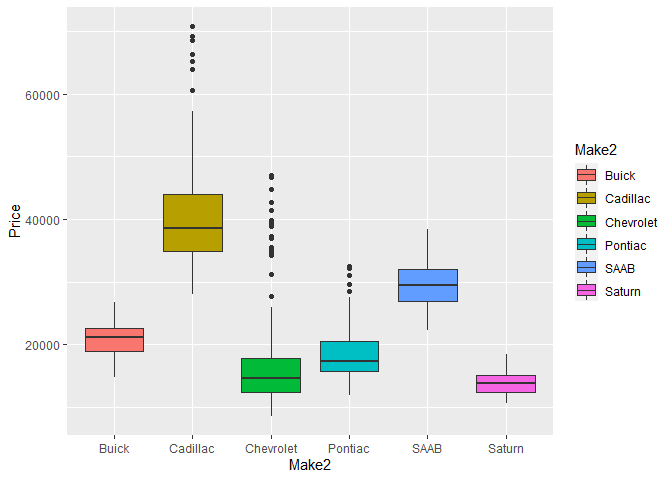
\includegraphics{Final-Reflection_files/figure-latex/unnamed-chunk-2-1.pdf}

\begin{Shaded}
\begin{Highlighting}[]
\CommentTok{\#Histograms}
\FunctionTok{ggplot}\NormalTok{(used\_cars2, }\FunctionTok{aes}\NormalTok{(}\AttributeTok{x =}\NormalTok{ Price)) }\SpecialCharTok{+}
  \FunctionTok{geom\_histogram}\NormalTok{(}\AttributeTok{fill =} \StringTok{"white"}\NormalTok{, }\AttributeTok{colour =} \StringTok{"black"}\NormalTok{) }\SpecialCharTok{+}
  \FunctionTok{facet\_wrap}\NormalTok{( }\SpecialCharTok{\textasciitilde{}}\NormalTok{ Make2, }\AttributeTok{ncol =} \DecValTok{2}\NormalTok{)}
\end{Highlighting}
\end{Shaded}

\begin{verbatim}
## `stat_bin()` using `bins = 30`. Pick better value with `binwidth`.
\end{verbatim}

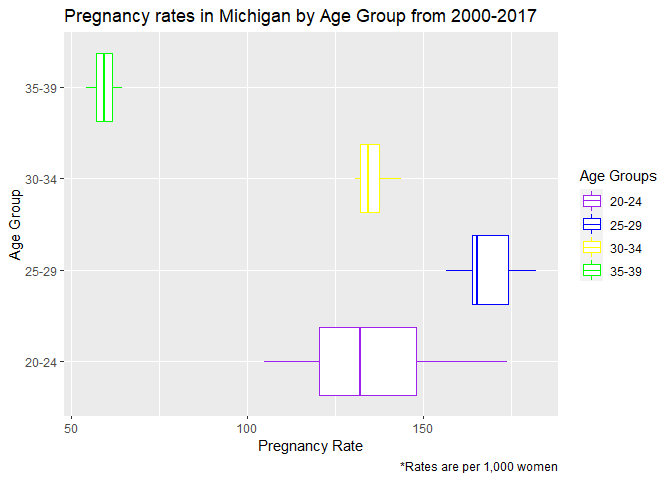
\includegraphics{Final-Reflection_files/figure-latex/unnamed-chunk-2-2.pdf}

\begin{Shaded}
\begin{Highlighting}[]
\CommentTok{\#Q{-}Q plots }
\NormalTok{used\_cars2 }\SpecialCharTok{\%\textgreater{}\%} 
  \FunctionTok{ggplot}\NormalTok{() }\SpecialCharTok{+}
  \FunctionTok{geom\_qq}\NormalTok{(}\AttributeTok{mapping =} \FunctionTok{aes}\NormalTok{(}\AttributeTok{sample =}\NormalTok{ Price)) }\SpecialCharTok{+}
  \FunctionTok{geom\_qq\_line}\NormalTok{(}\AttributeTok{mapping =} \FunctionTok{aes}\NormalTok{(}\AttributeTok{sample =}\NormalTok{ Price)) }\SpecialCharTok{+}
  \FunctionTok{facet\_wrap}\NormalTok{(}\FunctionTok{vars}\NormalTok{(Make2),}\AttributeTok{nrow =} \DecValTok{3}\NormalTok{)}
\end{Highlighting}
\end{Shaded}

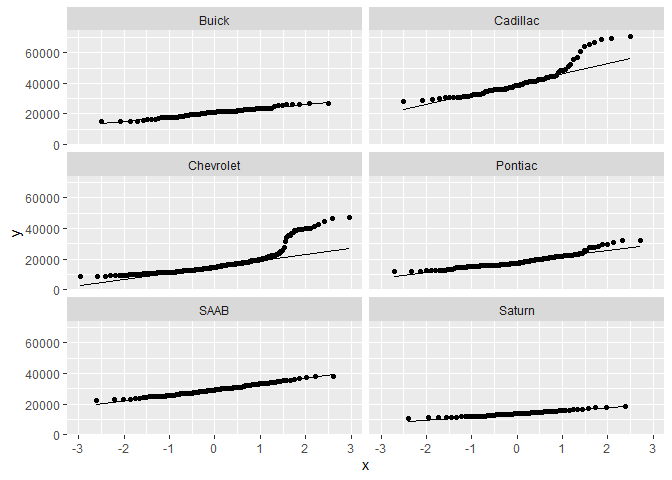
\includegraphics{Final-Reflection_files/figure-latex/unnamed-chunk-2-3.pdf}

\begin{itemize}
\tightlist
\item
  Writing R programs for simulation from probability models and
  randomization-based experiments
\end{itemize}

Honestly, I think this is the one part of the class that I really didn't
get a good handle on. I will have to go back through a couple of the
activities to show that I can accomplish this before this reflection is
officially do.

\begin{itemize}
\tightlist
\item
  Using source documentation and other resourced to troubleshoot and
  extend R programs.
\end{itemize}

Google has been my best friend in this class. Expectantly throughout the
final project. While going thought the process of trying to use leaflet
and shiny I have learned a lot from the Sinny app gallery and other
people on the internet that have gotten the same errors as I have. That
it the one nice things about R is most likely someone has run into the
same problems that you have. I have used a bunch of different discussion
board pages were people have put in there code to see if someone else
would be able to look at it and find the mistake. A lot of the time I
have the same exact error they do and am able to look in the comments to
see what others have suggested to fix the error. It is super rare that
no one has tried what you are doing before. So I am very grateful for
everyone that has struggled before me so that I can learn from their
mistakes as well. I also feel that getting errors also helps to get a
better understanding of how code should be written. I have extended my
knowledge of R extensively while trouble shooting and now have a much
better understanding of what needs to be included in specific commands
in order for them to run more smoothly.

\begin{itemize}
\tightlist
\item
  Write clear, efficient, and well-documented R programs
\end{itemize}

I think this will be best shown when I have finished the Shiny app side
of the final project. I am still working through getting all of my
sources together so that I can give credit to the code that has helped
me through the process of writing this app. So I know I will need to add
to this section once the final project is finished because as this
moment I don't have any other R programs and I feel would show what I
have accomplished in this aspect of the class.

\hypertarget{grade-and-other-thoughts}{%
\subsection{Grade and Other Thoughts}\label{grade-and-other-thoughts}}

I would give myself and A in this class, but I might change this if I am
not able to show my ability to write an R program for simulations from
probability models and randomization-based experiments. If I am able to
show this I will keep it at an A. However, If I look back to what I was
able to do at the beginning of the semester vs now I am amazed at what I
have accomplished. I am much more confident in what I am able to do in R
now vs the beginning of the semester. I also really appreciate the fact
that we have been given room to fail in this class. Knowing that I
haven't been solely focused on getting a specific grade I know I have
pushed myself to try and make the shiny app. I know I would have never
tried to take on such a task if I was so focused on the grade and by
pushing myself I have expaned my knowledge so much more.

\end{document}
